\begin{table}[t]
\caption{\textbf{Task suite of \ours,} including Adroit~\citep{rajeswaran2017dapg}, Bi-DexHands~\citep{chen2022bidexhands}, DexArt~\citep{bao2023dexart}, DexDeform~\citep{li2023dexdeform}, DexMV~\citep{qin2022dexmv}, HORA~\citep{qi2023hora}, MetaWorld~\citep{yu2020metaworld}, and our real robot tasks.
ActD: the highest action dimension for the domain. \#Demo: Number of expert demonstrations used for each task in the domain. Art: articulated objects. Deform: deformable objects.}
\label{table:task summary}
\vspace{-0.05in}
\resizebox{0.5\textwidth}{!}{%
\begin{tabular}{lcccccccc}
\toprule
\toprule
\multicolumn{7}{c}{\textbf{Simulation Benchmark (72 Tasks)}} \\
\midrule
 Domain & Robo  & Object  & Simulator & ActD & \#Task & \#Demo\\
 
\midrule
\textbf{Adroit} & Shadow & Rigid/Art & MuJoCo & 28 & 3 & 10\\


\textbf{Bi-DexHands} & Shadow & Rigid/Art &  IsaacGym & 52 & 6 & 10\\


\textbf{DexArt} & Allegro & Art & Sapien & 22 & 4 & 100 \\


\textbf{DexDeform} & Shadow & Deform & PlasticineLab & 52 & 6 & 10\\


\textbf{DexMV} & Shadow  & Rigid/Fluid & Sapien & 30 & 2 & 10\\


\textbf{HORA} & Allegro  & Rigid & IsaacGym & 16 & 1 & 100\\



\textbf{MetaWorld} & Gripper & Rigid/Art & MuJoCo & 4 & 50 & 10 \\


\toprule

% \textbf{Summary} & / & / & /  & 78 & / \\


\end{tabular}
}
\resizebox{0.5\textwidth}{!}{%
\begin{tabular}{lcccclcccc}
\multicolumn{6}{c}{\textbf{Real Robot Benchmark (4 Tasks) }} \\
\midrule

Task & Robo & Object &  ActD & \#Demo & Description\\

\midrule
\textbf{Roll-Up} & Allegro & Deform & 22 & 40 & Wrap plasticine to make a roll-up\\

\textbf{Dumpling} & Allegro & Deform & 22 & 40 & Wrap plasticine and pinch with fingers\\

\textbf{Drill} & Allegro & Rigid & 22 & 40 & Grasp the drill and touch the cube\\

% \textbf{Scissors} & Allegro & Art & 22 & 40 & Pick the scissors towards flowers\\

\textbf{Pour} & Gripper & Rigid & 7 & 40 & Pick the bowl, pour, and place \\
\bottomrule
\bottomrule
\end{tabular}
}
% 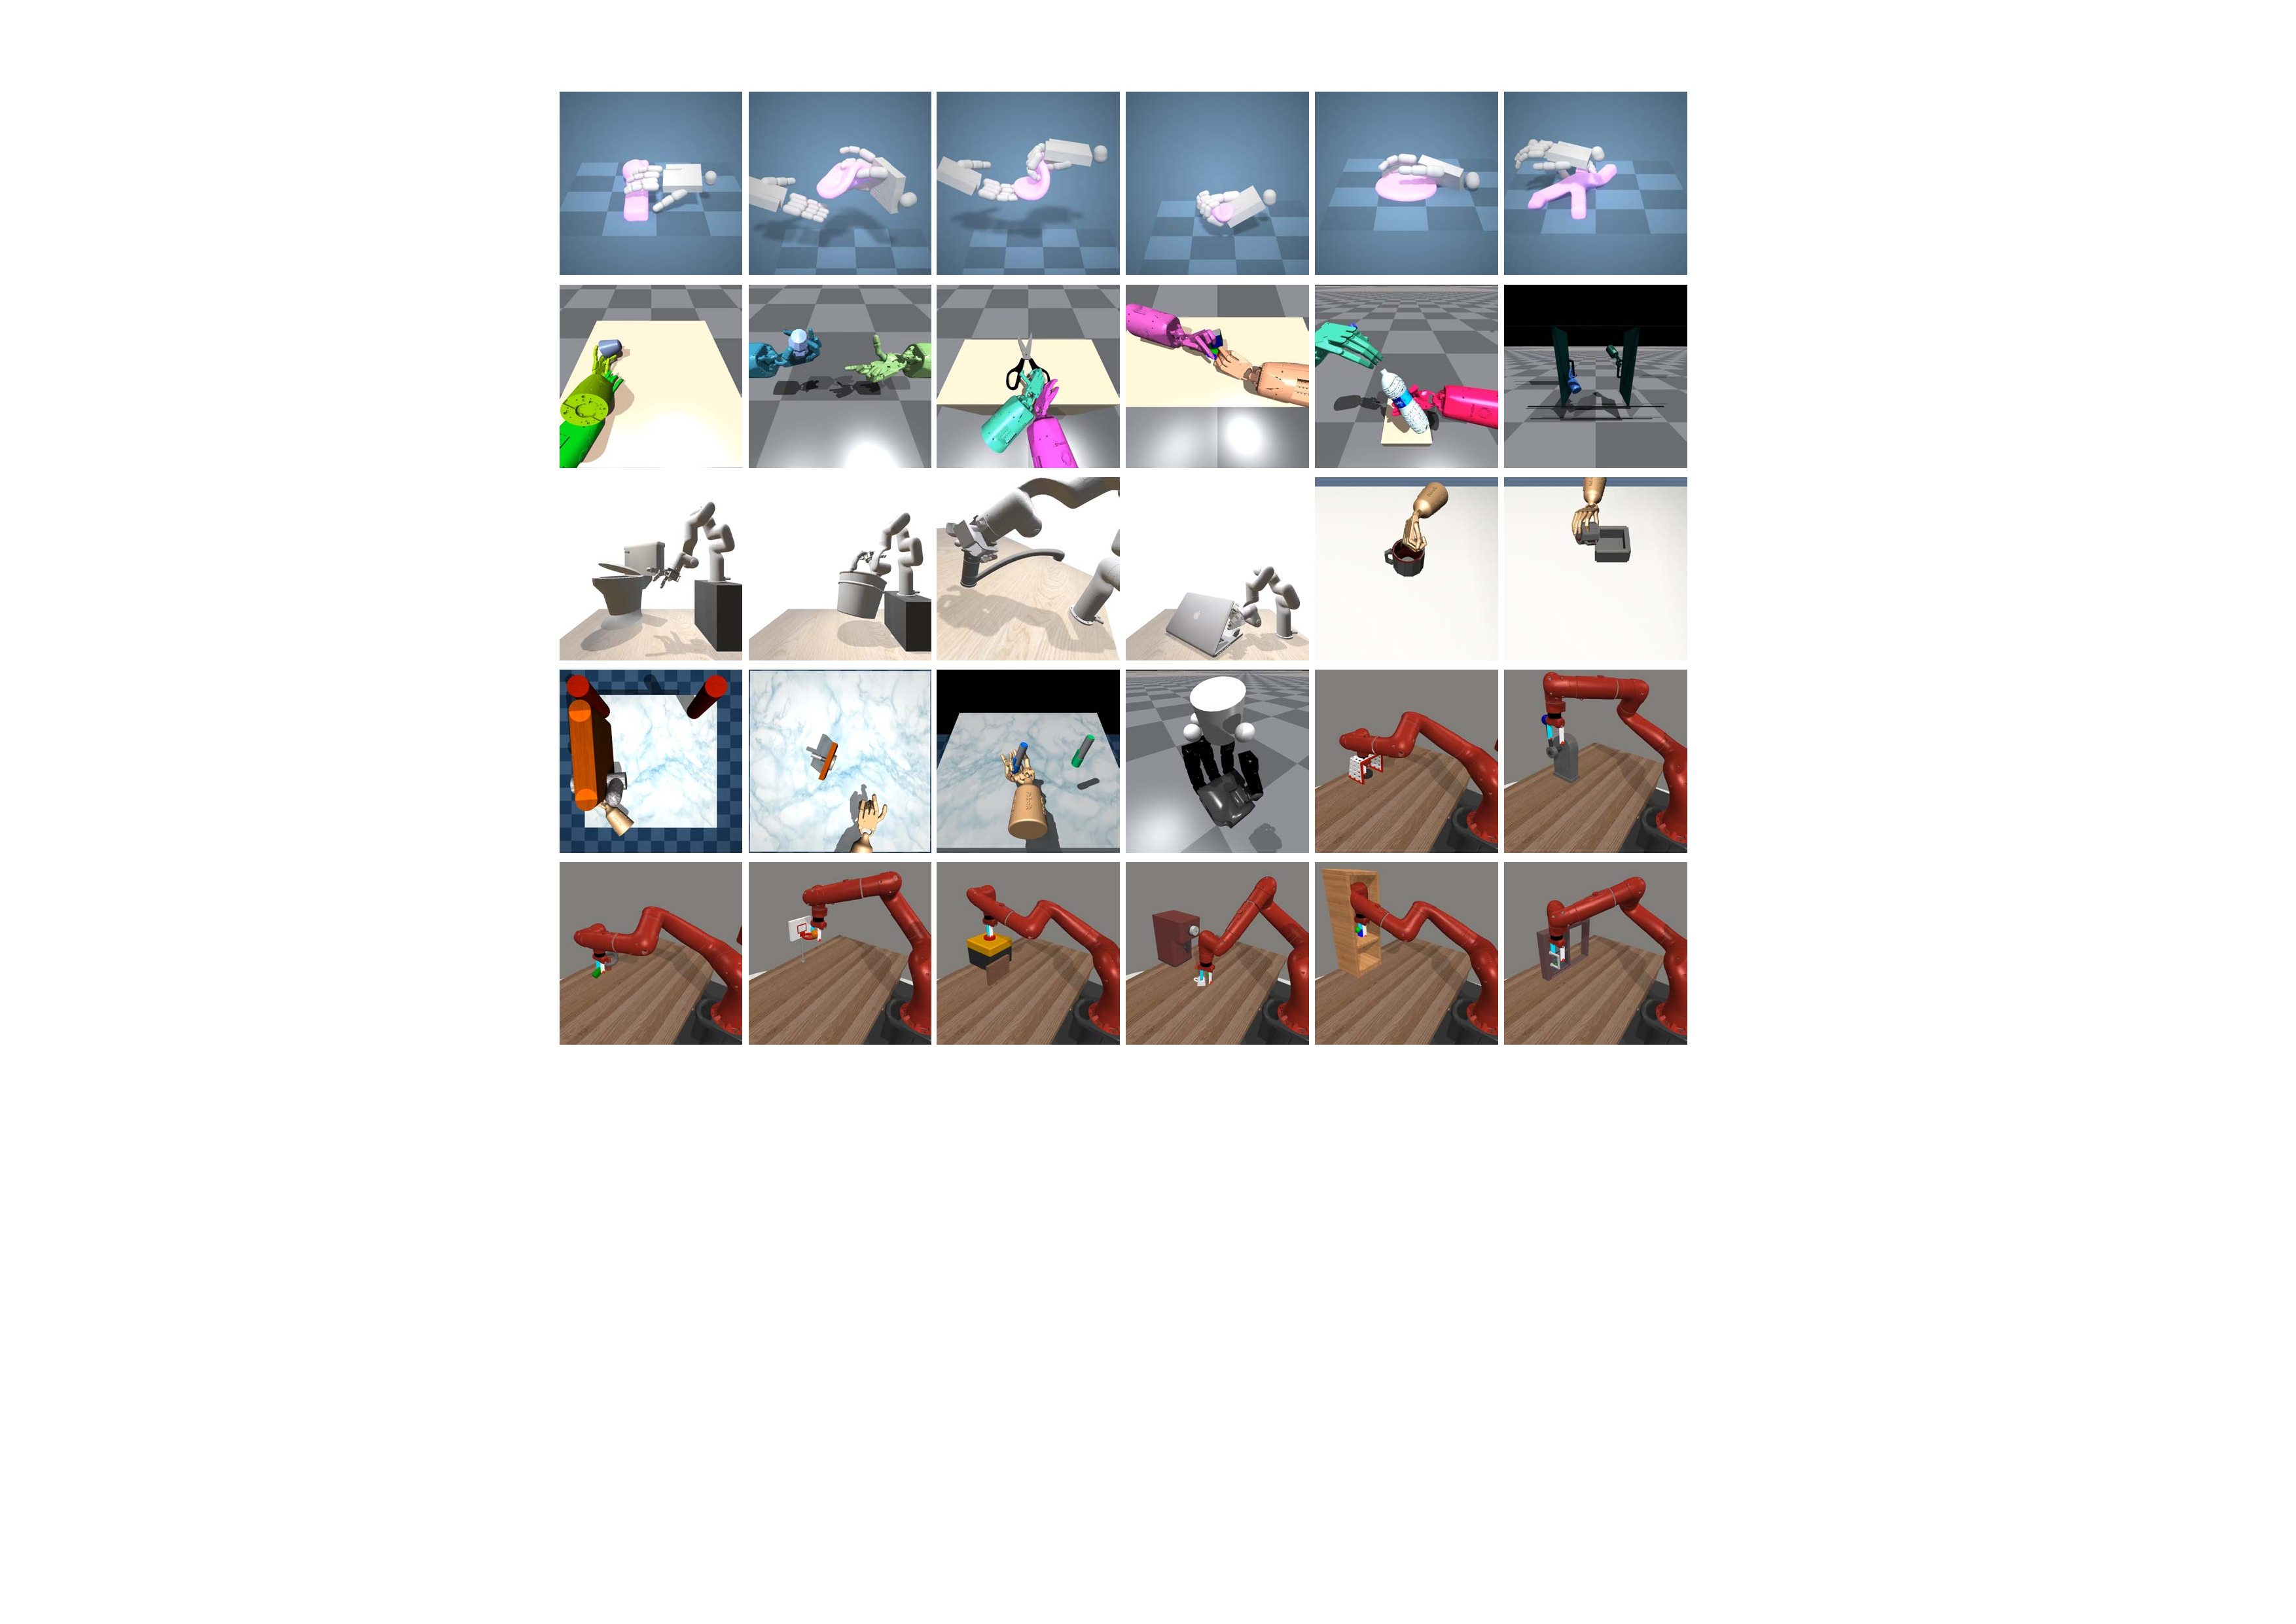
\includegraphics[width=0.5\textwidth]{figures/task_visualization_compress.pdf}
\vspace{-0.2in}
 \end{table}







